\documentclass{standalone}
\usepackage{tikz}
\usepackage{amsmath}
\begin{document}

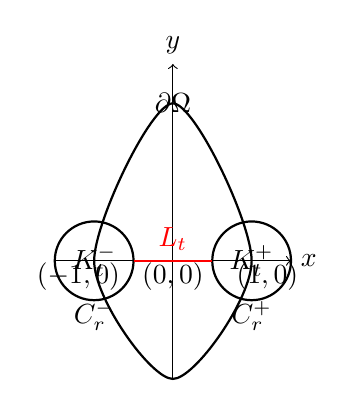
\begin{tikzpicture}
    % Define styles for curves and lines
    \tikzset{
        curve/.style={thick},
        dashedcurve/.style={thick, dashed},
        redcurve/.style={thick, red},
    }
    
    % Draw the outer shape
    \draw[curve] plot [smooth cycle] coordinates {(-1,0) (0,2) (1,0) (0,-1.5)};
    
    % Draw the x and y axes
    \draw[->] (-1.5,0) -- (1.5,0) node[right] {$x$};
    \draw[->] (0,-1.5) -- (0,2.5) node[above] {$y$};
    
    % Draw the inner circles
    \draw[curve] (-1,0) circle (0.5) node at (-1,0) {$K^-_t$};
    \draw[curve] (1,0) circle (0.5) node at (1,0) {$K^+_t$};
    
    % Draw the line L_t
    \draw[redcurve] (-0.5,0) -- (0.5,0) node[midway, above] {$L_t$};
    
    % Draw additional annotations
    \node at (0,2) {$\partial \Omega$};
    \node at (0,-0.2) {$(0,0)$};
    \node at (-1.2,-0.2) {$(-1,0)$};
    \node at (1.2,-0.2) {$(1,0)$};
    \node at (-1,-0.7) {$C^-_r$};
    \node at (1,-0.7) {$C^+_r$};
\end{tikzpicture}

\end{document}